\section{Understanding the Hyperparameter Loss Surface Across Scales}
\label{sec:understanding-the-hyperparameter-loss-surface-across-scales}

Throughout this section, we will make use of the same experiments we ran in the previous section. Note, that we additionally fit a noisy quadratic distribution to each scale for our analysis. 
%
We show that models become less sensitive to hyperparameters as they scale (\S\ref{sec:understanding-the-hyperparameter-loss-surface-across-scales:hyperparameter-tuning-gets-easier-with-scale}). This phenomenon traces back to the hyperparameter loss surface: larger scale makes it lower dimensional (\S\ref{sec:understanding-the-hyperparameter-loss-surface-across-scales:the-hyperparameter-loss-surface-becomes-lower-dimensional}). These facts influence how we design experiments (\S\ref{sec:understanding-the-hyperparameter-loss-surface-across-scales:implications-for-small-scale-experiments}): small scales require extensive search, while large scales are easy to adapt.

\subsection{Hyperparameter Tuning Gets Easier with Scale}
\label{sec:understanding-the-hyperparameter-loss-surface-across-scales:hyperparameter-tuning-gets-easier-with-scale}


\begin{figure}
    \centering
    \begin{minipage}{0.24\linewidth}
        \centering
        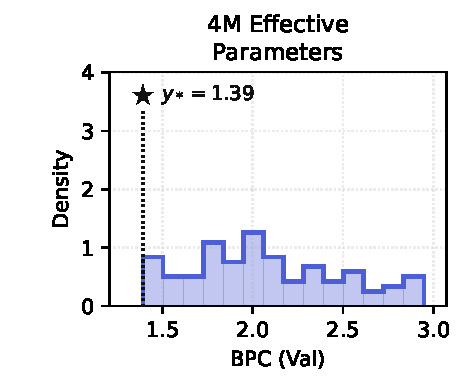
\includegraphics[width=\linewidth]{figures/panel1_dist_4M.pdf}\\
        {\small (a) Scores at 4M}
    \end{minipage}
    \hfill
    \begin{minipage}{0.24\linewidth}
        \centering
        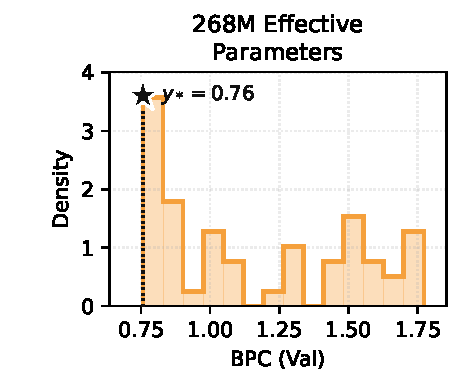
\includegraphics[width=\linewidth]{figures/panel2_dist_268M.pdf}\\
        {\small (b) Scores at 268M}
    \end{minipage}
    \hfill
    \begin{minipage}{0.24\linewidth}
        \centering
        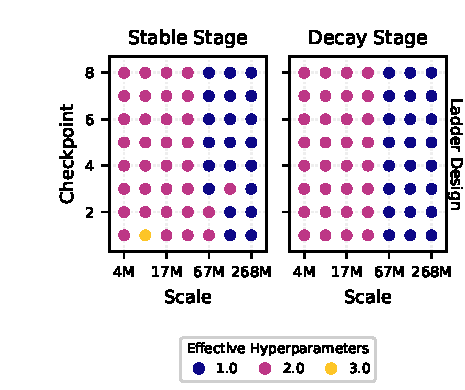
\includegraphics[width=\linewidth]{figures/panel3_effective_hyperparameters.pdf}\\
        {\small (c) Effective hyperparameters}
    \end{minipage}
    \hfill
    \begin{minipage}{0.24\linewidth}
        \centering
        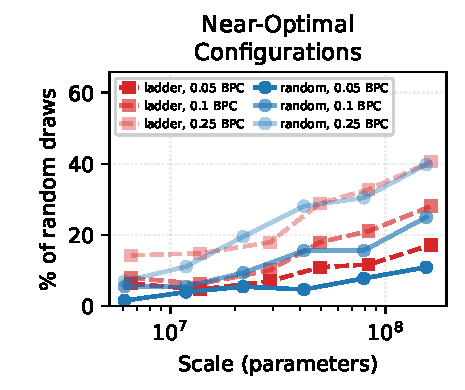
\includegraphics[width=\linewidth]{figures/panel4_hit_rate.pdf}\\
        {\small (d) Near-optimal configurations}
    \end{minipage}
    \caption{
        \emph{Smaller scales are more sensitive to hyperparameter tuning.}
        We visualize the distribution over validation losses at the end of training from random
        search, in bits per character. \textbf{(a)} At 4M the
        distribution is broad and flat, so fewer configurations land near the best achievable loss,
        $y_*$.  \textbf{(b)} At 268M, the density concentrates into a peak close to $y_*$, three times higher
        on the shared axis than the 4M scale. These results demonstrate that more hyperparameter configurations land next to the optimum at larger scales and that smaller scales are more sensitive to hyperparameter tuning. \textbf{(c)} The effective hyperparameter count ($\gamma$) is the intrinsic dimension of the hyperparameter loss surface. We estimate $\gamma$ at each parameter--data budget by fitting the noisy quadratic distribution to results from random search. With and without learning rate decay, $\gamma$ trends lower as parameters increase, while increasing data has much less of an effect.
        \textbf{(d)} The percentage of configurations within $0.1$ bits per character of $y_*$ grows from 7.9\% to 28.1\%
        between 4M and 134M.
    }
    \label{fig:hyperparameter-sensitivity-loss-surface}
\end{figure}

With scale, good configurations become more common; thus, larger models trained longer are easier to tune.

\paragraph{Near-optimal configurations fill a larger fraction of the space.} The effort required to find a good configuration depends on the fraction of the space they take up. We can measure this volume via Monte Carlo integration: sample configurations uniformly and check what percent land near the optimum. This procedure is exactly random search. \Cref{fig:hyperparameter-sensitivity-loss-surface}(a,b) shows how the score distribution changes with scale: as models grow, the distribution concentrates on the best achievable loss and the density forms a peak. Thus scale makes models easier to tune.


\paragraph{Hyperparameter sensitivity decreases through both parameters and data.} We show in \Cref{fig:hyperparameter-sensitivity-loss-surface}(d) that the percentage of configurations within different loss thresholds of the optimal loss increases with scale for both the ladder and random designs.
Additionally, neither parameters nor data alone is responsible for this decrease in sensitivity; the effect comes from both. In fact, \Cref{fig:hyperparameter-sensitivity-decreases-through-both-parameters-and-data} shows the minimum, 10th, and 25th percentile validation losses from random search and illustrates how sensitivity decreases across each. The gap from the 25th percentile to the minimum directly measures sensitivity because a small gap means that a quarter of all draws are already close to optimal. Scaling one dimension while the other is held small lowers the loss and slightly moves this gap, but scaling one while the other is large collapses it. 

\subsection{The Effective Number of Hyperparameters Decreases with Scale}
\label{sec:understanding-the-hyperparameter-loss-surface-across-scales:the-hyperparameter-loss-surface-becomes-lower-dimensional}


Intuitively, a model with more hyperparameters is harder to tune; in practice, models can have many while their effective number is still low. Formally, the effective number of hyperparameters ($\gamma$) is the surface's intrinsic dimension at the optimum, a major determinant of tuning difficulty \citep{lourie2025hyperparameter}. We estimate $\gamma$ at each parameter--data budget by fitting a noisy quadratic to the tail from random search (all losses below a threshold, $\theta$). We show these estimates against model size in \Cref{fig:hyperparameter-sensitivity-loss-surface}(d), where \textbf{larger models have fewer effective hyperparameters}, dropping to one. Moreover, checkpoints across training largely share the same intrinsic dimension, while increasing parameters clearly reduces $\gamma$. 

% Therefore, parameters more than data drive the decrease in effective hyperparameters.

Thus the effective number of hyperparameters shrinks as parameters grow. Data seems to have less effect. Interestingly, prior work found the effective hyperparameters remains constant when using the same search space across different architectures \citep[\S D]{lourie2025hyperparameter}. It seems counter-intuitive that $\gamma$ depends on scale but not architecture. Moreover, scale's effect might change under an alternative parametrization, such as maximum update \citep{yang2021tuning}. All these factors likely influence $\gamma$ at some point, our results refine a prior for typical regimes. Better understanding these limits would be a valuable direction for future work.

\subsection{Implications for Small-Scale Experiments}
\label{sec:understanding-the-hyperparameter-loss-surface-across-scales:implications-for-small-scale-experiments}

The HP loss surface is not a black box; it has rich qualitative structure. We showed empirically that as parameters and data grow, it gets easier to optimize, good configurations fill the space, and the intrinsic dimension goes down. Good reason to hope that there is a simple structure underpinning the HP loss surface, which we may exploit when optimizing at large scales. After all, \citep{lourie2025hyperparameter} already showed the noisy quadratic to be a good model for the outcomes of HP optimization at a single scale. Our efforts to model the HP surface across scales however showed no consistent success. We describe several interpretable models in \S\ref{app:interpretable-models-of-the-hyperparameter-loss-surface} (and tried many more). While simple models capture coarse features of the surface, none characterize its finer details. The simplest model, one ignoring how HPs change with scale, is already a strong baseline. This outcome agrees with the qualitative picture: extrapolating to larger scales, HPs have less impact and little variation is left to model.
%
As a result, we treat HP optimization independently per scale.